\cleardoublepage

\chapter{Sides}

%%%%%%%%%%%%%%%%%%%%%%%%%%%%%%%%%%%%%%%%%%%%%%%%%%%%%%%%%%%%%%%%%%%%%%%%%%%
%%%%%%%%%%%%%%%%%%%%%%%%%%%%%%%%%%%%%%%%%%%%%%%%%%%%%%%%%%%%%%%%%%%%%%%%%%%
%%%%%%%%%%%%%%%%%%%%%%%%%%%%%%%%%%%%%%%%%%%%%%%%%%%%%%%%%%%%%%%%%%%%%%%%%%%
%%%%%%%%%%%%%%%%%%%%%%%%%%%%%%%%%%%%%%%%%%%%%%%%%%%%%%%%%%%%%%%%%%%%%%%%%%%
%%%%%%%%%%%%%%%%%%%%%%%%%%%%%%%%%%%%%%%%%%%%%%%%%%%%%%%%%%%%%%%%%%%%%%%%%%%

\section{Présentation}

\textit{Sides} est un projet de gestion de titres développé par Sopra Group, plus particulièrement par l'agence de Clermont Ferrand.
Il permet de produire des passeports ou des cartes d'identités pour une dizaine de différents gouvernement comme les Philippines, la Belgique, Monaco, \ldots
\\

Pour chacun des pays et titres, une application a été développée.
Plutôt que de redévelopper la même application, un nouveau projet a vu le jour : \textit{SITI}.
Cette solution pourra ensuite être vendue à divers pays sans avoir à la ré-implémenter à nouveau.

Actuellement l'équipe Sides n'effectue que de la tiers maintenance applicative (TMA) sur les différentes applications existantes.
L'objectif est de corriger les bugs éventuels ou d'ajouter de nouvelles fonctionnalités.

%%%%%%%%%%%%%%%%%%%%%%%%%%%%%%%%%%%%%%%%%%%%%%%%%%%%%%%%%%%%%%%%%%%%%%%%%%%
%%%%%%%%%%%%%%%%%%%%%%%%%%%%%%%%%%%%%%%%%%%%%%%%%%%%%%%%%%%%%%%%%%%%%%%%%%%
%%%%%%%%%%%%%%%%%%%%%%%%%%%%%%%%%%%%%%%%%%%%%%%%%%%%%%%%%%%%%%%%%%%%%%%%%%%
%%%%%%%%%%%%%%%%%%%%%%%%%%%%%%%%%%%%%%%%%%%%%%%%%%%%%%%%%%%%%%%%%%%%%%%%%%%
%%%%%%%%%%%%%%%%%%%%%%%%%%%%%%%%%%%%%%%%%%%%%%%%%%%%%%%%%%%%%%%%%%%%%%%%%%%

\section{Chargement d'empreintes}

%%%%%%%%%%%%%%%%%%%%%%%%%%%%%%%%%%%%%%%%%%%%%%%%%%%%%%%%%%%%%%%%%%%%%%%%%%%
%%%%%%%%%%%%%%%%%%%%%%%%%%%%%%%%%%%%%%%%%%%%%%%%%%%%%%%%%%%%%%%%%%%%%%%%%%%
%%%%%%%%%%%%%%%%%%%%%%%%%%%%%%%%%%%%%%%%%%%%%%%%%%%%%%%%%%%%%%%%%%%%%%%%%%%

\subsection{Contexte}

L'application Sides à destination des Philippines permet la gestion de passeports.
Ces passeports nécessitent la lecture des empreintes du porteur pour être valides.
Lorsque les porteurs sont des personnes diplomatiques ou haut placées, celles-ci désireraient ne pas perdre de temps lors de création ou renouvellement de titres.

Pour satisfaire ces exigences, une personne du gouvernement munie d'un ordinateur portable, de l'application Sides et du périphérique va effectuer la saisie des empreintes sur le lieu désiré : ville plus proche, lieu de travail, \ldots

%%%%%%%%%%%%%%%%%%%%%%%%%%%%%%%%%%%%%%%%%%%%%%%%%%%%%%%%%%%%%%%%%%%%%%%%%%%
%%%%%%%%%%%%%%%%%%%%%%%%%%%%%%%%%%%%%%%%%%%%%%%%%%%%%%%%%%%%%%%%%%%%%%%%%%%
%%%%%%%%%%%%%%%%%%%%%%%%%%%%%%%%%%%%%%%%%%%%%%%%%%%%%%%%%%%%%%%%%%%%%%%%%%%

\subsection{Contrôle de la date}

La première version de cette fonctionnalité permettait l'importation des empreintes les plus récentes présentes dans la base de données pour créer un nouveau passeport.
Les empreintes peuvent venir d'une ancienne demande ou avoir été saisies pour une personne diplomatique comme expliqué précédemment.

Pour sécuriser l'application et le chargement d'anciennes empreintes, l'évolution de la fonctionnalité a pour objectif de contrôler la date d'importation des empreintes dans la base de données.
\\

Pour réaliser ce contrôle, j'ai dû étudier le fonctionnement de l'application pour comprendre le processus de chargement des empreintes dans une nouvelle demande de passeport.

%%%%%%%%%%%%%%%%%%%%%%%%%%%%%%%%%%%%%%%%%%%%%%%%%%%%%%%%%%%%%%%%%%%%%%%%%%%
%%%%%%%%%%%%%%%%%%%%%%%%%%%%%%%%%%%%%%%%%%%%%%%%%%%%%%%%%%%%%%%%%%%%%%%%%%%
%%%%%%%%%%%%%%%%%%%%%%%%%%%%%%%%%%%%%%%%%%%%%%%%%%%%%%%%%%%%%%%%%%%%%%%%%%%
%%%%%%%%%%%%%%%%%%%%%%%%%%%%%%%%%%%%%%%%%%%%%%%%%%%%%%%%%%%%%%%%%%%%%%%%%%%
%%%%%%%%%%%%%%%%%%%%%%%%%%%%%%%%%%%%%%%%%%%%%%%%%%%%%%%%%%%%%%%%%%%%%%%%%%%

\section{Les certificats}

%%%%%%%%%%%%%%%%%%%%%%%%%%%%%%%%%%%%%%%%%%%%%%%%%%%%%%%%%%%%%%%%%%%%%%%%%%%
%%%%%%%%%%%%%%%%%%%%%%%%%%%%%%%%%%%%%%%%%%%%%%%%%%%%%%%%%%%%%%%%%%%%%%%%%%%
%%%%%%%%%%%%%%%%%%%%%%%%%%%%%%%%%%%%%%%%%%%%%%%%%%%%%%%%%%%%%%%%%%%%%%%%%%%

\subsection{Contexte}

La gestion des identités de personnes, au niveau national, est un domaine très sensible qui requière une sécurité élevée des systèmes informatiques.
La solution permettant de sécuriser les données consiste à chiffrer ou signer les données échangées, garantissant ainsi que les données ne pourront être découverte ou qu'elles n'ont pas été modifiée ou envoyées par une personne tiers. Ce chiffrement s'effectue grâce à des certificats.

%%%%%%%%%%%%%%%%%%%%%%%%%%%%%%%%%%%%%%%%%%%%%%%%%%%%%%%%%%%%%%%%%%%%%%%%%%%
%%%%%%%%%%%%%%%%%%%%%%%%%%%%%%%%%%%%%%%%%%%%%%%%%%%%%%%%%%%%%%%%%%%%%%%%%%%
%%%%%%%%%%%%%%%%%%%%%%%%%%%%%%%%%%%%%%%%%%%%%%%%%%%%%%%%%%%%%%%%%%%%%%%%%%%

\subsubsection{Le chiffrement}

Pour assurer que personne ne puisse découvrir le message échangé entre deux personnes il est nécessaire de les chiffrer.
Le fonctionnement est le suivant, schématisé par la figure \ref{chiffrement} :
\begin{enumerate}
	\item Bob possède une paire de clé publique/privée, et Alice désire envoyer un message à Bob ;
	\item Bob envoie sa clé publique à Alice ;
	\item Alice chiffre son message grâce à cette clé publique ;
	\item Alice envoie ensuite son message chiffré à Bob ;
	\item Bob déchiffre le message chiffré grâce à sa clé privée. Personne d'autre ne peut le faire car il est le seul à posséder la clé privée.
\end{enumerate}
\begin{figure}[!h]
	\center
	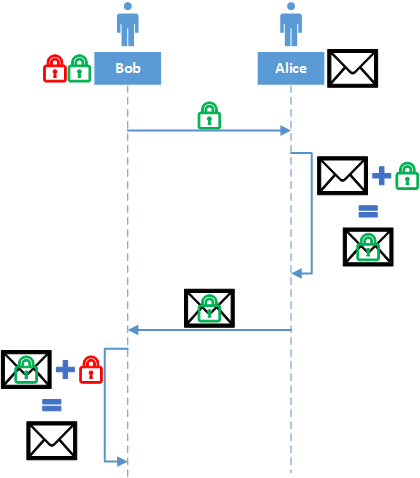
\includegraphics[width=0.7\textwidth]{img/chiffrement.png}
	\caption{Échange d'une message chiffré}
	\label{chiffrement}
\end{figure}
~~\\

La sécurité est basée sur deux principes : le chiffrement et la confidentialité.

Si l'algorithme de chiffrement est trop faible ou que la clé est trop petite alors les données peuvent être découverte par "brute force", c'est à dire en essayant toutes les combinaisons possibles.

Si la clé privée du certificat est découverte alors les données seront instantanément déchiffrées.
Il est donc nécessaire de renouveler les clés régulièrement.

%%%%%%%%%%%%%%%%%%%%%%%%%%%%%%%%%%%%%%%%%%%%%%%%%%%%%%%%%%%%%%%%%%%%%%%%%%%

\subsubsection{La signature}

La signature numérique permet de vérifier l'authenticité et la non-modification d'un message.

Le fonctionnement est le suivant, schématisé par la figure \ref{signature} :
\begin{enumerate}
	\item Bob hache le message, puis chiffre ce hash avec sa clé privée, ce qui produit la signature du message ;
	\item Bob envoie à Alice le message, la clé publique et la signature ;
	\item Alice hache le message, et déchiffre la signature du message grâce à la clé publique. Ensuite elle compare les deux valeurs, qui seront égales si le message n'a pas été modifié et a été chiffré avec la clé privée associée à la clé publique.
\end{enumerate}
\begin{figure}[!h]
	\center
	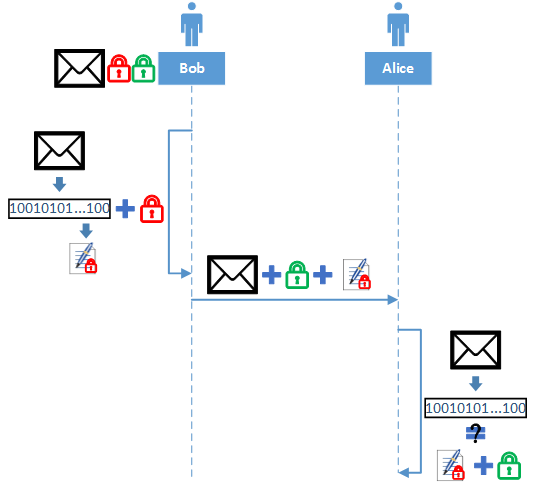
\includegraphics[width=0.7\textwidth]{img/signature.png}
	\caption{Échange d'un message signé}
	\label{signature}
\end{figure}
~~\\

%%%%%%%%%%%%%%%%%%%%%%%%%%%%%%%%%%%%%%%%%%%%%%%%%%%%%%%%%%%%%%%%%%%%%%%%%%%

\subsubsection{Le certificat}

Un certificat est composé de :
\begin{itemize}
	\item une clé publique, et éventuellement la clé privée associée ;
	\item des informations sur le propriétaire ;
	\item une signature.
\end{itemize}

Les certificats sont signés par une autorité de certification.
Seule l'autorité de certification racine est auto-signée.

%%%%%%%%%%%%%%%%%%%%%%%%%%%%%%%%%%%%%%%%%%%%%%%%%%%%%%%%%%%%%%%%%%%%%%%%%%%

\subsubsection{La PKI}

Une \textit{infrastructure à clés publiques}, aussi appelé \textit{public key infrastructure}, permet la gestion de grandes quantités de certificats ou clés publiques.
Elle fournie des services de création, de publication et de révocation de certificats.








PKI
Application : utilisation de certificats
SOD : permet de générer des certificats sans PKI pour tester les applications

%%%%%%%%%%%%%%%%%%%%%%%%%%%%%%%%%%%%%%%%%%%%%%%%%%%%%%%%%%%%%%%%%%%%%%%%%%%
%%%%%%%%%%%%%%%%%%%%%%%%%%%%%%%%%%%%%%%%%%%%%%%%%%%%%%%%%%%%%%%%%%%%%%%%%%%
%%%%%%%%%%%%%%%%%%%%%%%%%%%%%%%%%%%%%%%%%%%%%%%%%%%%%%%%%%%%%%%%%%%%%%%%%%%

\subsection{Documentation SOD}

%%%%%%%%%%%%%%%%%%%%%%%%%%%%%%%%%%%%%%%%%%%%%%%%%%%%%%%%%%%%%%%%%%%%%%%%%%%
%%%%%%%%%%%%%%%%%%%%%%%%%%%%%%%%%%%%%%%%%%%%%%%%%%%%%%%%%%%%%%%%%%%%%%%%%%%
%%%%%%%%%%%%%%%%%%%%%%%%%%%%%%%%%%%%%%%%%%%%%%%%%%%%%%%%%%%%%%%%%%%%%%%%%%%

\subsection{Projet de test du SOD}



~~\\--------------------------------------~~\\
TODO:
SOD : documentation + exemples